\documentclass{beamer}

\usetheme{Warsaw}

\beamertemplatenavigationsymbolsempty

\usepackage[utf8]{inputenc}
\usepackage[ngerman]{babel}

\usepackage{amsmath}
\usepackage[ruled]{algorithm2e}

\useoutertheme{infolines}

\resetcounteronoverlays{algocf}

\usepackage{tikz}

\usetikzlibrary{positioning, shapes, arrows, tikzmark, calc}

\usepackage{varwidth}
\usepackage{tikz-3dplot}

\usepackage{picture}

\def\stdItemSep{.5em}

\def\HiLi{\leavevmode\rlap{\hbox to \hsize{\color{yellow!50}\leaders\hrule height .8\baselineskip depth .5ex\hfill}}}

\newcommand{\newSectionFrame}[1]
{
	\begin{frame}
		\vfill
		\centering
		\begin{beamercolorbox}[sep=8pt,center,shadow=true,rounded=true]{title}
			\usebeamerfont{title}#1\par%
		\end{beamercolorbox}
		\vfill
	\end{frame}
}

\AtBeginSection[]
{
	\newSectionFrame{\insertsectionhead}
}

\AtBeginSubsection[]
{
	\newSectionFrame{\insertsubsectionhead}
}

\AtBeginSubsubsection[]
{
	\newSectionFrame{\insertsubsubsectionhead}
}

\title{Big Data Praktikum: ER with Bit Arrays}
\author{Moritz Engelmann, Maik Fröbe}
\date{31.07.2017}

\parindent 0pt

\newcounter{image_index_counter} 

\begin{document}

\begin{frame}
	\vfill
	\centering
	\begin{beamercolorbox}[sep=8pt,center,shadow=true,rounded=true]{title}
		\usebeamerfont{title}
		Speed up Entity Resolution with Bit Arrays\\
		\par%
	\end{beamercolorbox}
	\vfill
	\textbf{Big Data Praktikum}\\
	\textbf{SS 17}\\
	\vfill
	Moritz Engelmann\\
	Maik Fröbe
	\vfill
	\hspace*{5.1cm}31.07.2017
\end{frame}

\begin{frame}
	\tableofcontents
\end{frame}

\section{Einführung}

\begin{frame}
	\frametitle{Problembeschreibung}

	\begin{itemize}
		\setlength\itemsep{\stdItemSep}
		\item Eingabe
		\begin{itemize}
			\setlength\itemsep{\stdItemSep}
			\vspace*{\stdItemSep}
			\item 2 Mengen von Personen
			\item Verhältnis 80:20
			\vspace*{1cm}
		\end{itemize}
		\item Ziel
		\begin{itemize}
			\setlength\itemsep{\stdItemSep}
			\vspace*{\stdItemSep}
			\item finden ähnlicher Personen in beiden Datensätzen
			\vspace*{2cm}
		\end{itemize}
		\item Anforderungen
		\begin{itemize}
			\setlength\itemsep{\stdItemSep}
			\vspace*{\stdItemSep}
			\item Bestimmung der Ähnlichkeit mit Jaccard-Index 
			\item $jaccard(A, B)$ $=$ $\frac{|A \cap B|}{|A \cup B|}$
		\end{itemize}
	\end{itemize}
	
	\begin{tikzpicture}[overlay]
		\node (start) at (8.5, 6.6) {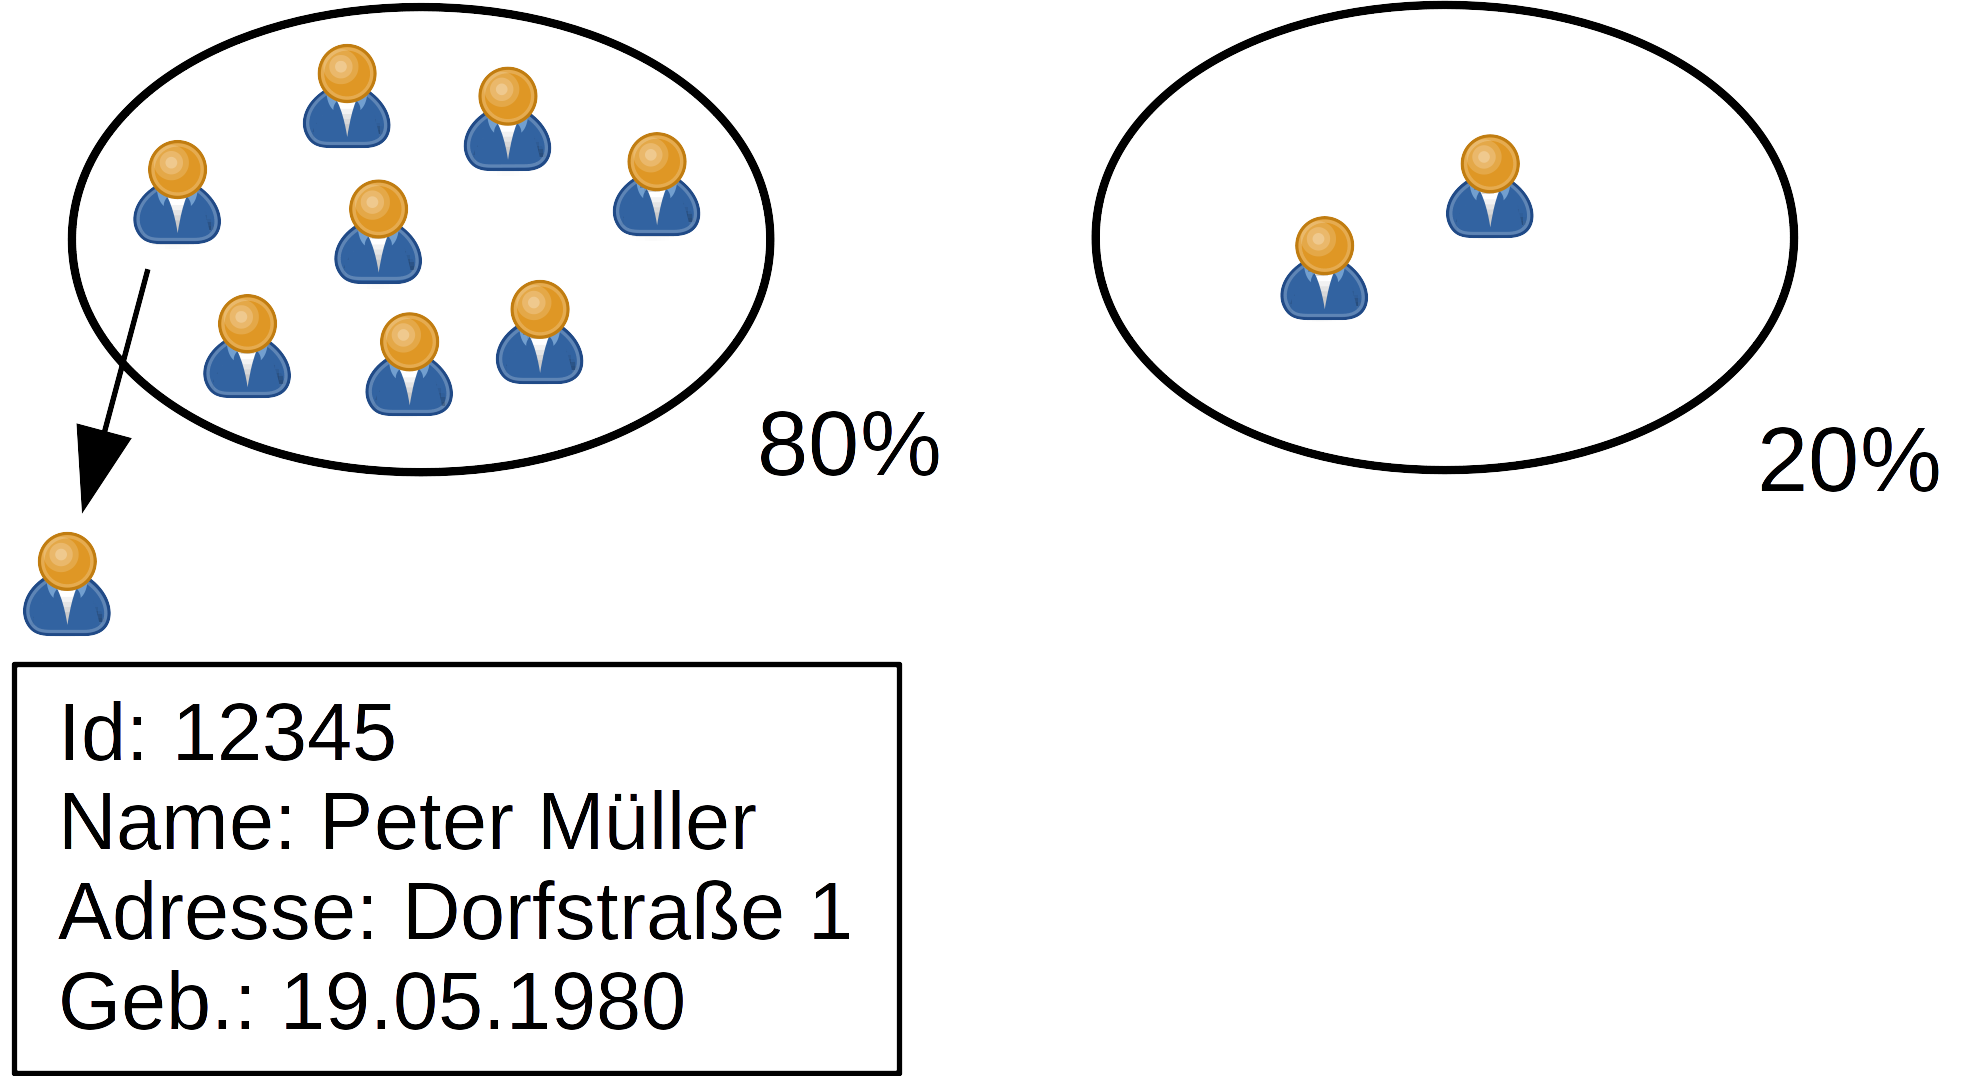
\includegraphics[width=0.5\textwidth]{Bilder/Eingabe.png}};
		\node (start) at (5.5, 3.2) {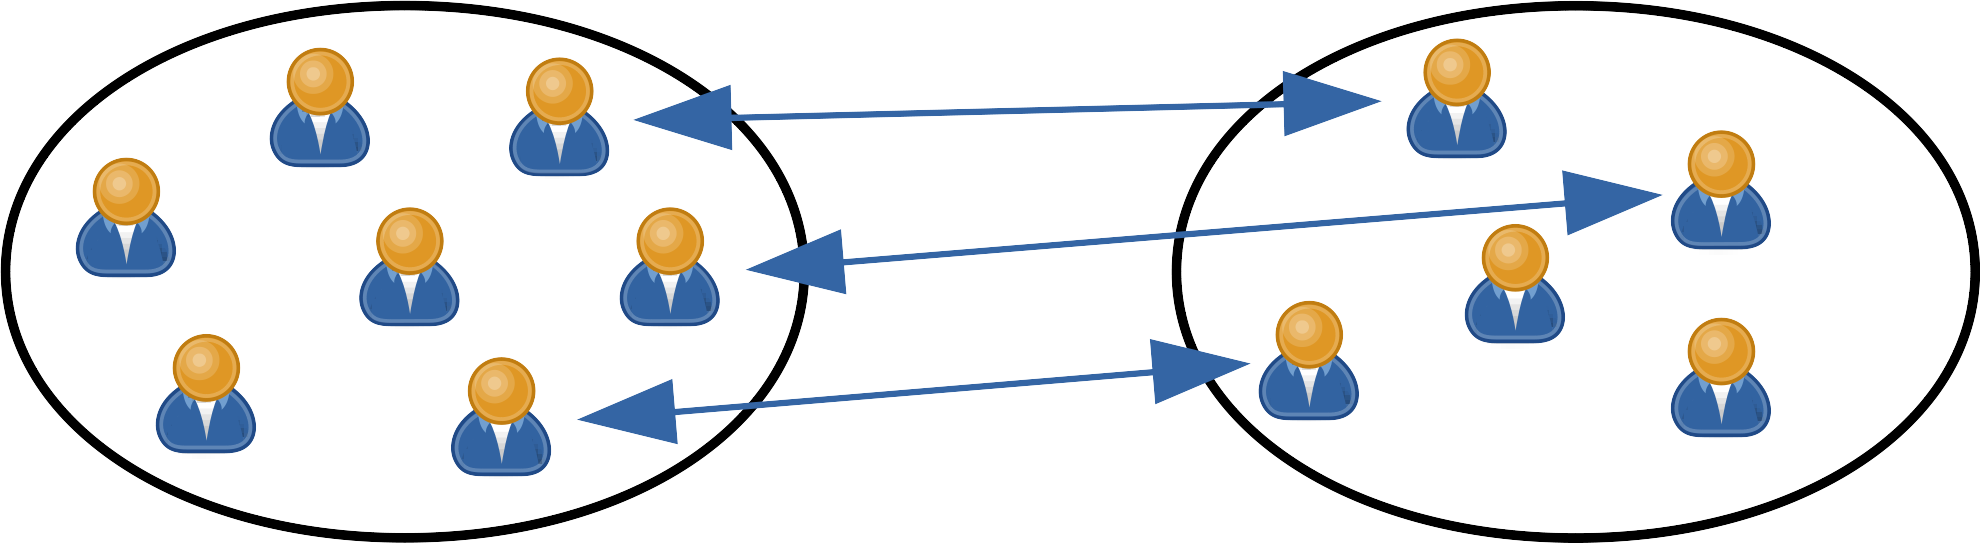
\includegraphics[width=0.5\textwidth]{Bilder/Problem.png}};
	\end{tikzpicture}
\end{frame}

\begin{frame}
	\frametitle{Framework zur Entity-Resolution}

	\begin{itemize}
		\setlength\itemsep{\stdItemSep}
		\item vollständig Parametrisierbar
		\item Modular
		\item Start der Entity-Resolution mit:
		\begin{itemize}
			\setlength\itemsep{\stdItemSep}
			\vspace*{\stdItemSep}
			\item Transformation: Person $\rightarrow$ $V$
			\item Ähnlichkeit: $V \times V$ $\rightarrow$ $[0,1]$
			\item $n$ (Größe der $n$-Gramme)
			\item Threshold
			\item \ldots
		\end{itemize}
		\item sequentieller Nested-Loop
		\begin{itemize}
			\setlength\itemsep{\stdItemSep}
			\vspace*{\stdItemSep}
			\item Vollständige Berechnung der Ähnlichkeit für kartesisches Produkt
		\end{itemize}
	\end{itemize}
\end{frame}


\begin{frame}
	\frametitle{Importphase}
	\begin{center}
	\vspace*{-.2cm}
	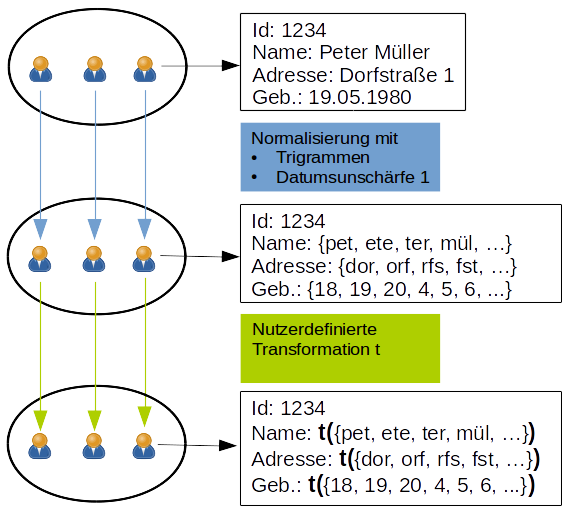
\includegraphics[height=0.9\textheight]{Bilder/Importphase.png}
	\end{center}
\end{frame}


\section{Ansätze zur Entity-Resolution}

\subsection{Trivialer Ansatz}
\begin{frame}
	\vspace*{-0.15cm}
	\hspace*{-.35cm} \textbf{\underline{Transformation:}}
	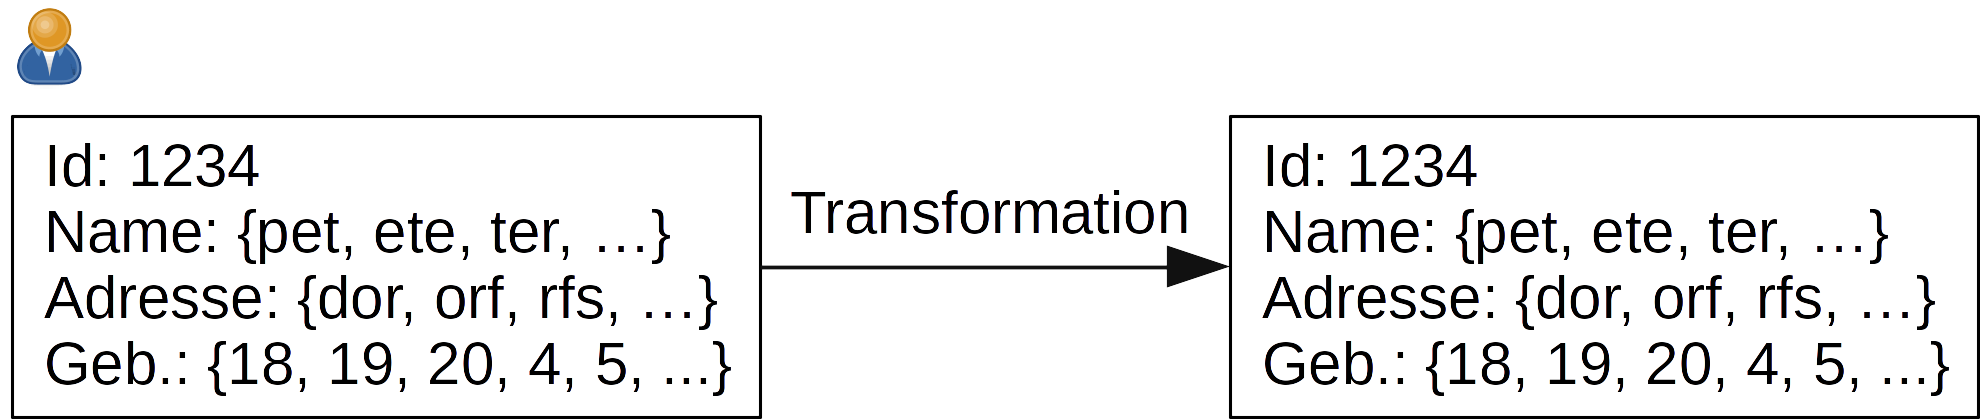
\includegraphics[width=1.01\textwidth]{Bilder/Transformation_Strings.png}
	\vspace*{0.35cm}

	\hspace*{-.35cm} \textbf{\underline{Ähnlichkeitsfunktion:}}
	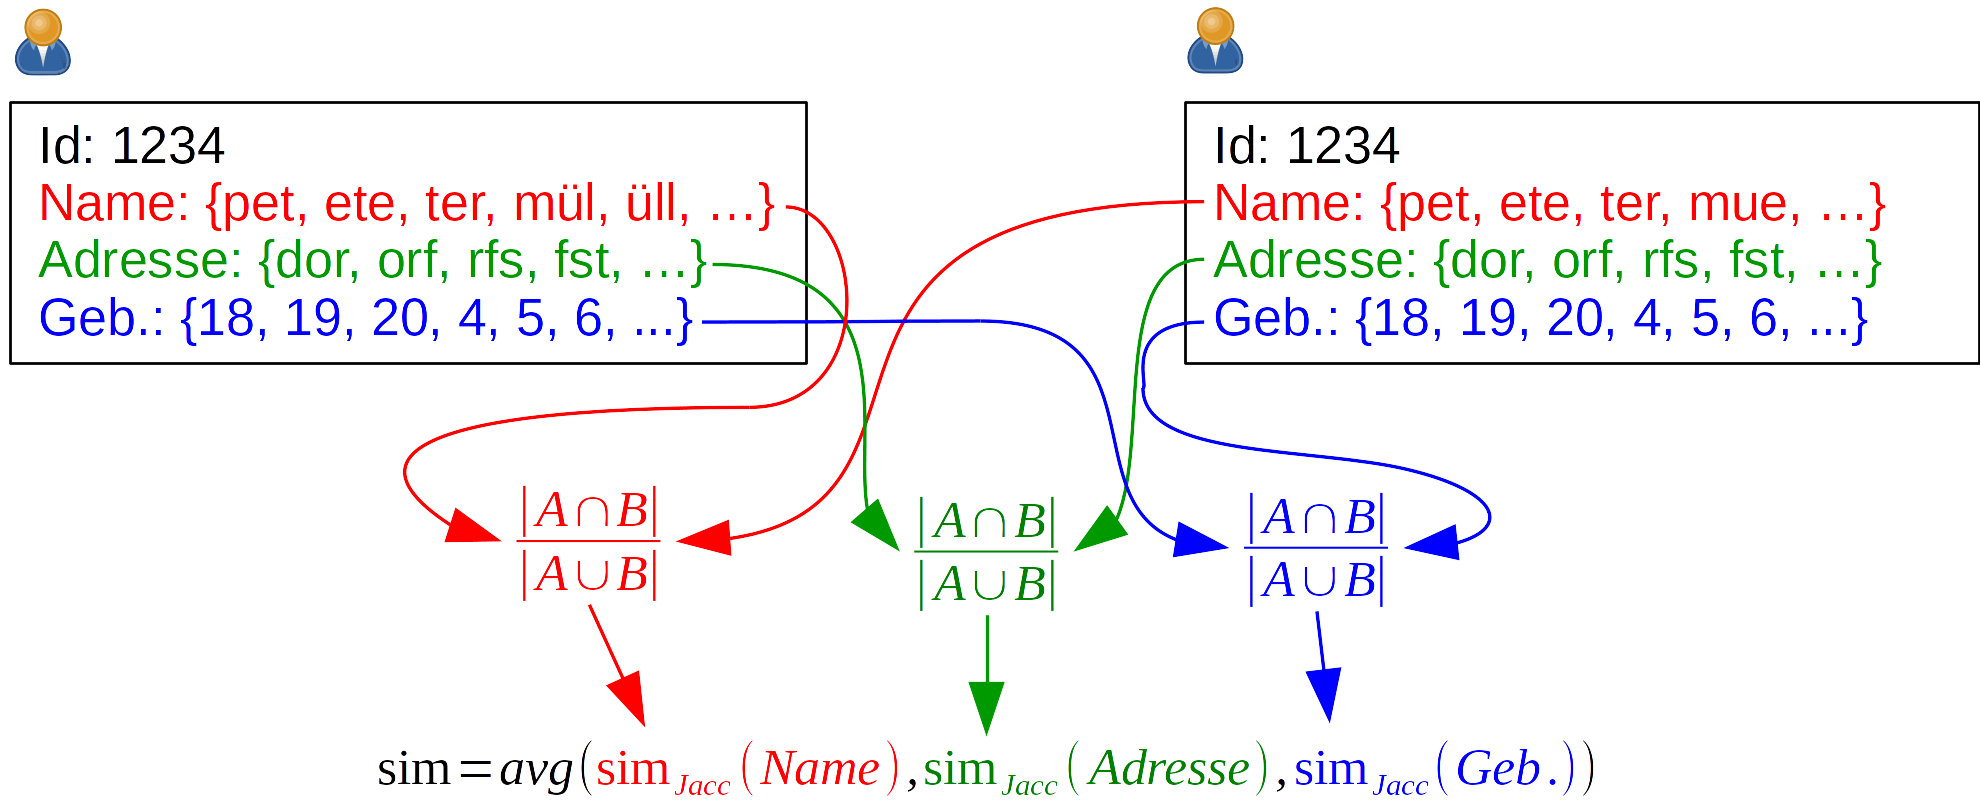
\includegraphics[width=1.01\textwidth]{Bilder/sim_strings.png}
\end{frame}

\subsection{Sortier-Ansatz}
\begin{frame}
	\begin{itemize}
		\setlength\itemsep{\stdItemSep}
		\item Analog zu Sort-Merge-Verbund\footnotemark
		\begin{itemize}
			\setlength\itemsep{\stdItemSep}
			\vspace*{\stdItemSep}
			\item Während Import: Sortiere Mengen
			\item Während ER: Berechne Kardinalität der Schnittmenge in $\mathcal{O}(n)$
			\begin{itemize}
				\setlength\itemsep{\stdItemSep}
				\vspace*{\stdItemSep}
				\item Schritthaltende Traversierung der sortierten Mengen
			\end{itemize}
		\end{itemize}
	\end{itemize}

	\footnotetext[1]{Siehe Vorlesung Implementierung von Datenbanksystemen}
\end{frame}

\subsection{Bit-Array-Ansatz}
\begin{frame}
	\frametitle{Einschub: Bloom-Filter}

	\uncover<1-1>
	{
		\begin{tikzpicture}[overlay]
			\node (start) at (6.1, -0.47) {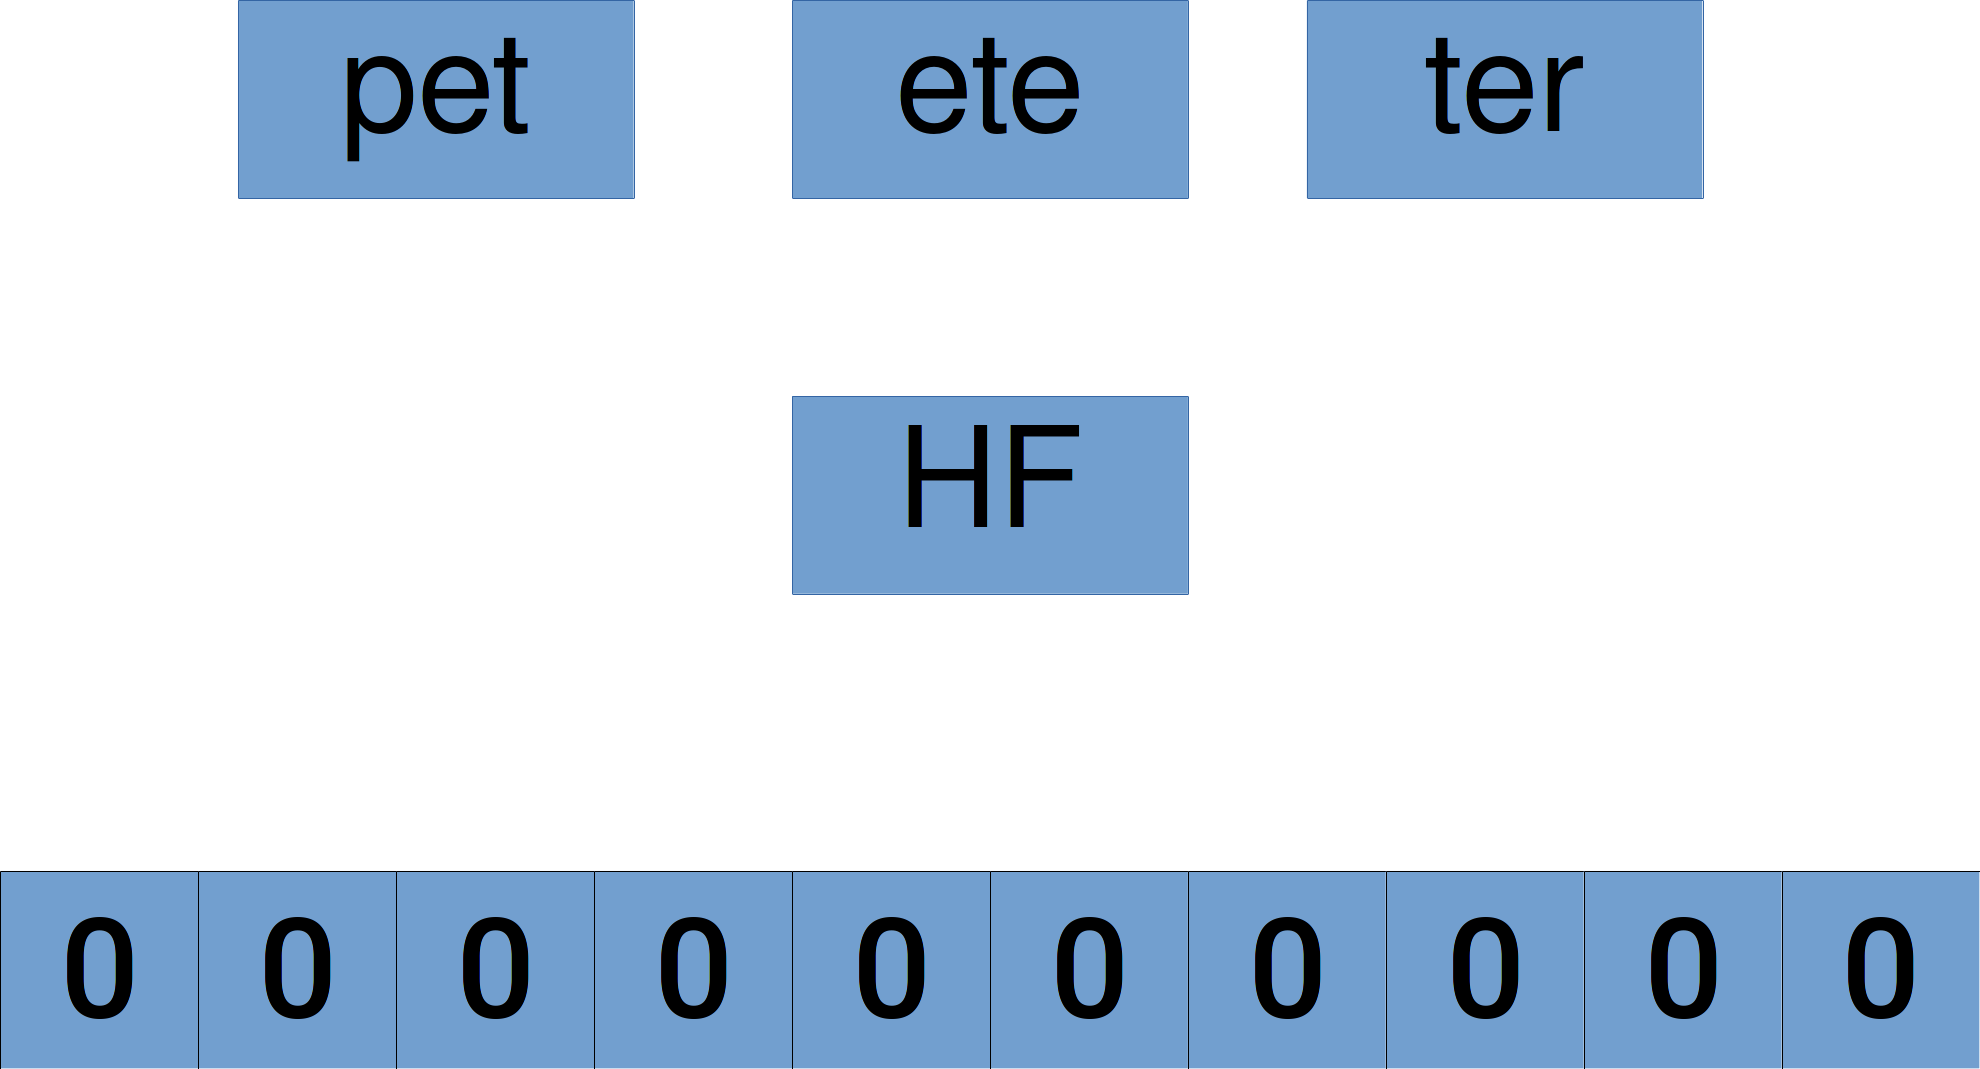
\includegraphics[width=0.9\textwidth]{Bilder/bloomfilter_example_insert_01.png}};
		\end{tikzpicture}
	}

	\uncover<2-2>
	{
		\begin{tikzpicture}[overlay]
			\node (start) at (6.1, 0) {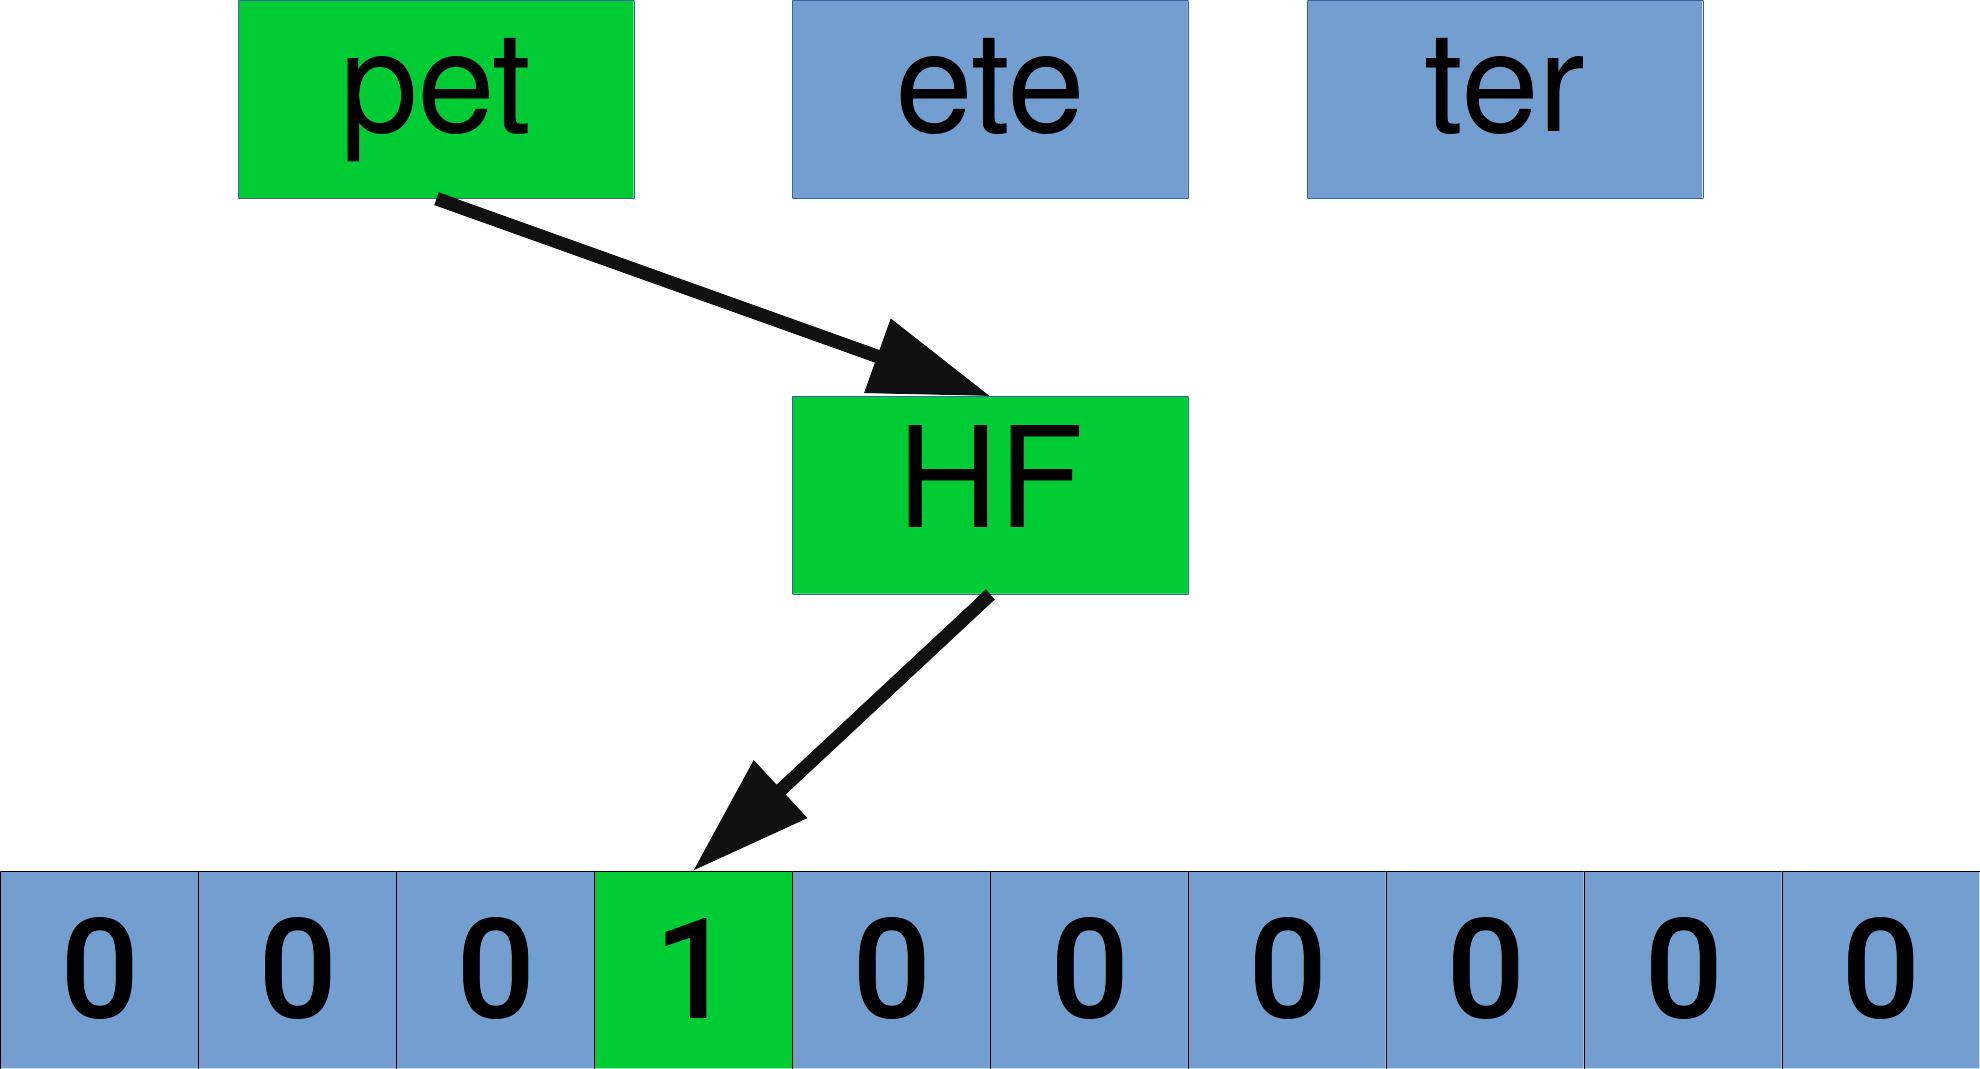
\includegraphics[width=0.9\textwidth]{Bilder/bloomfilter_example_insert_02.png}};
		\end{tikzpicture}
	}

	\uncover<3-3>
	{
		\begin{tikzpicture}[overlay]
			\node (start) at (6.1, 0.47) {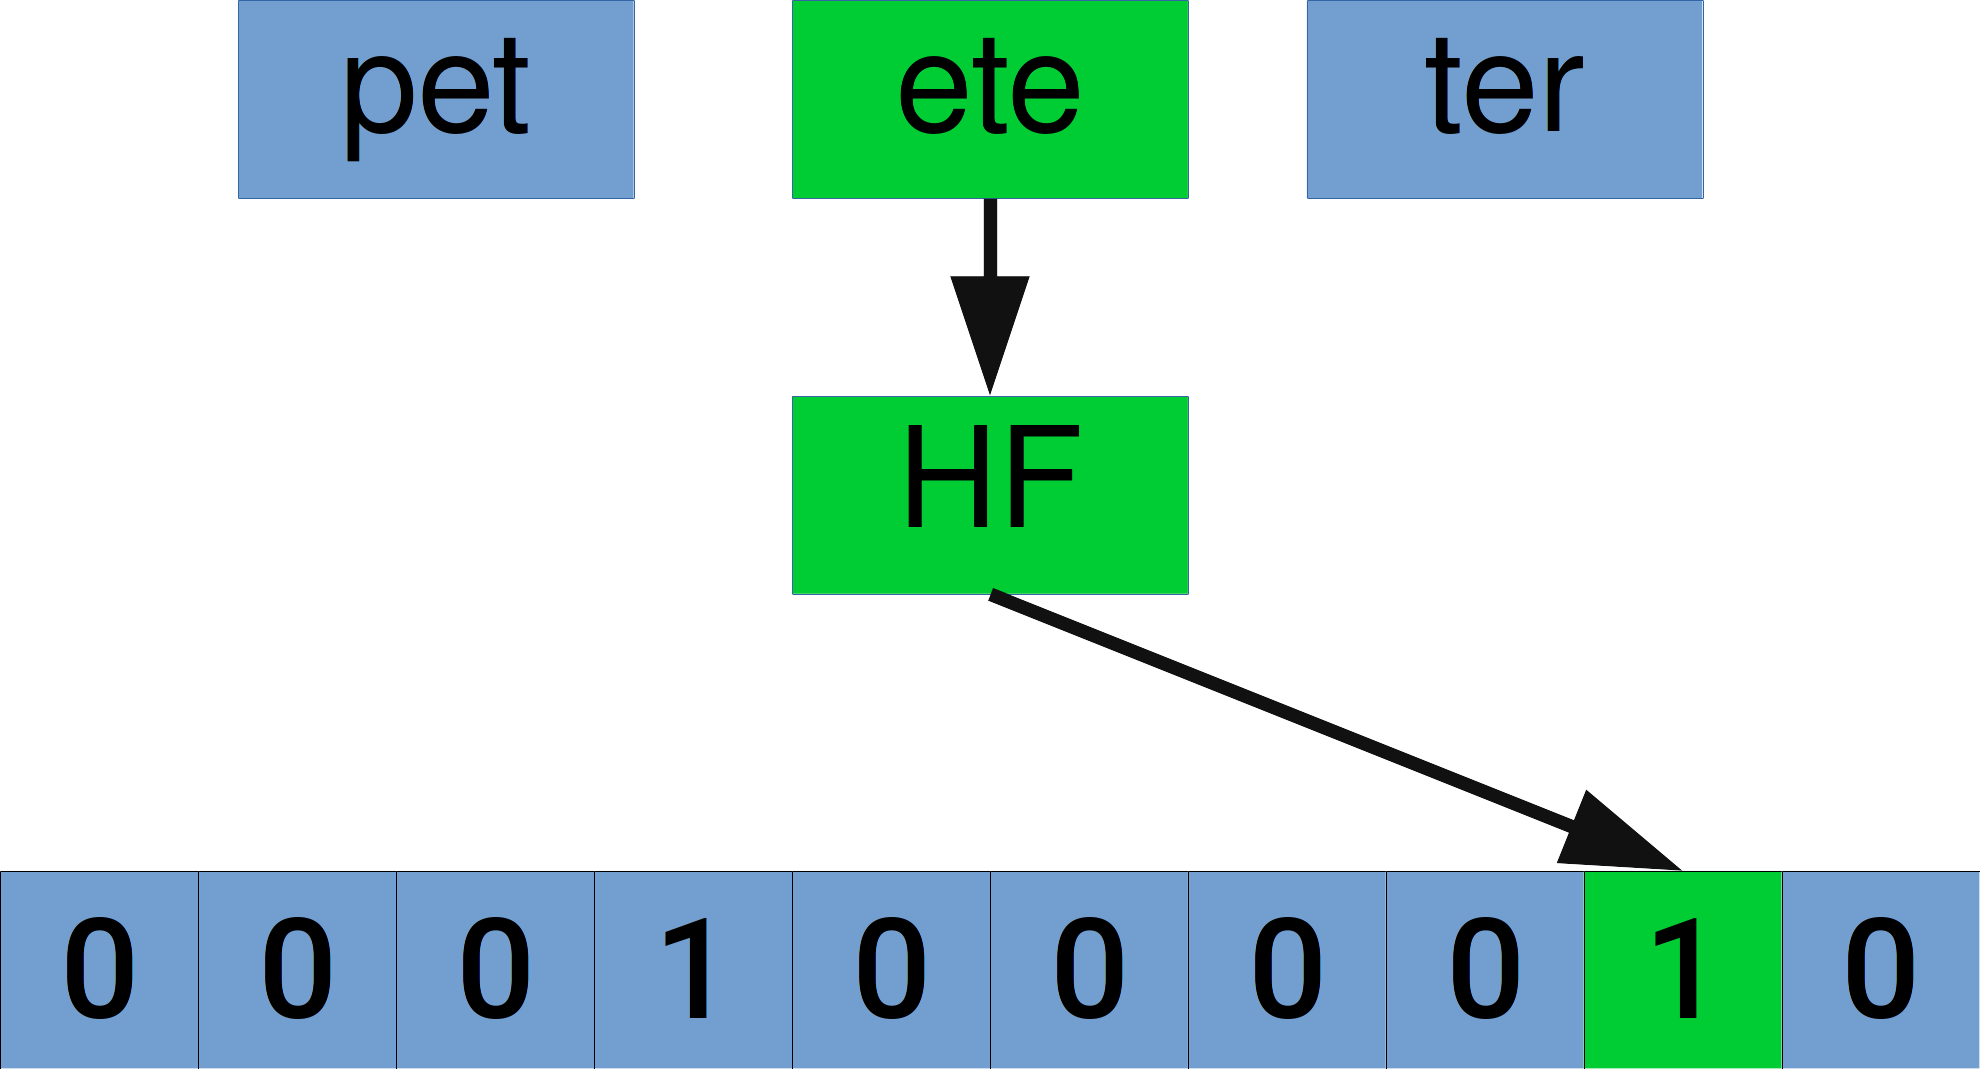
\includegraphics[width=0.9\textwidth]{Bilder/bloomfilter_example_insert_03.png}};
		\end{tikzpicture}
	}

	\uncover<4-4>
	{
		\begin{tikzpicture}[overlay]
			\node (start) at (6.1, 0.94) {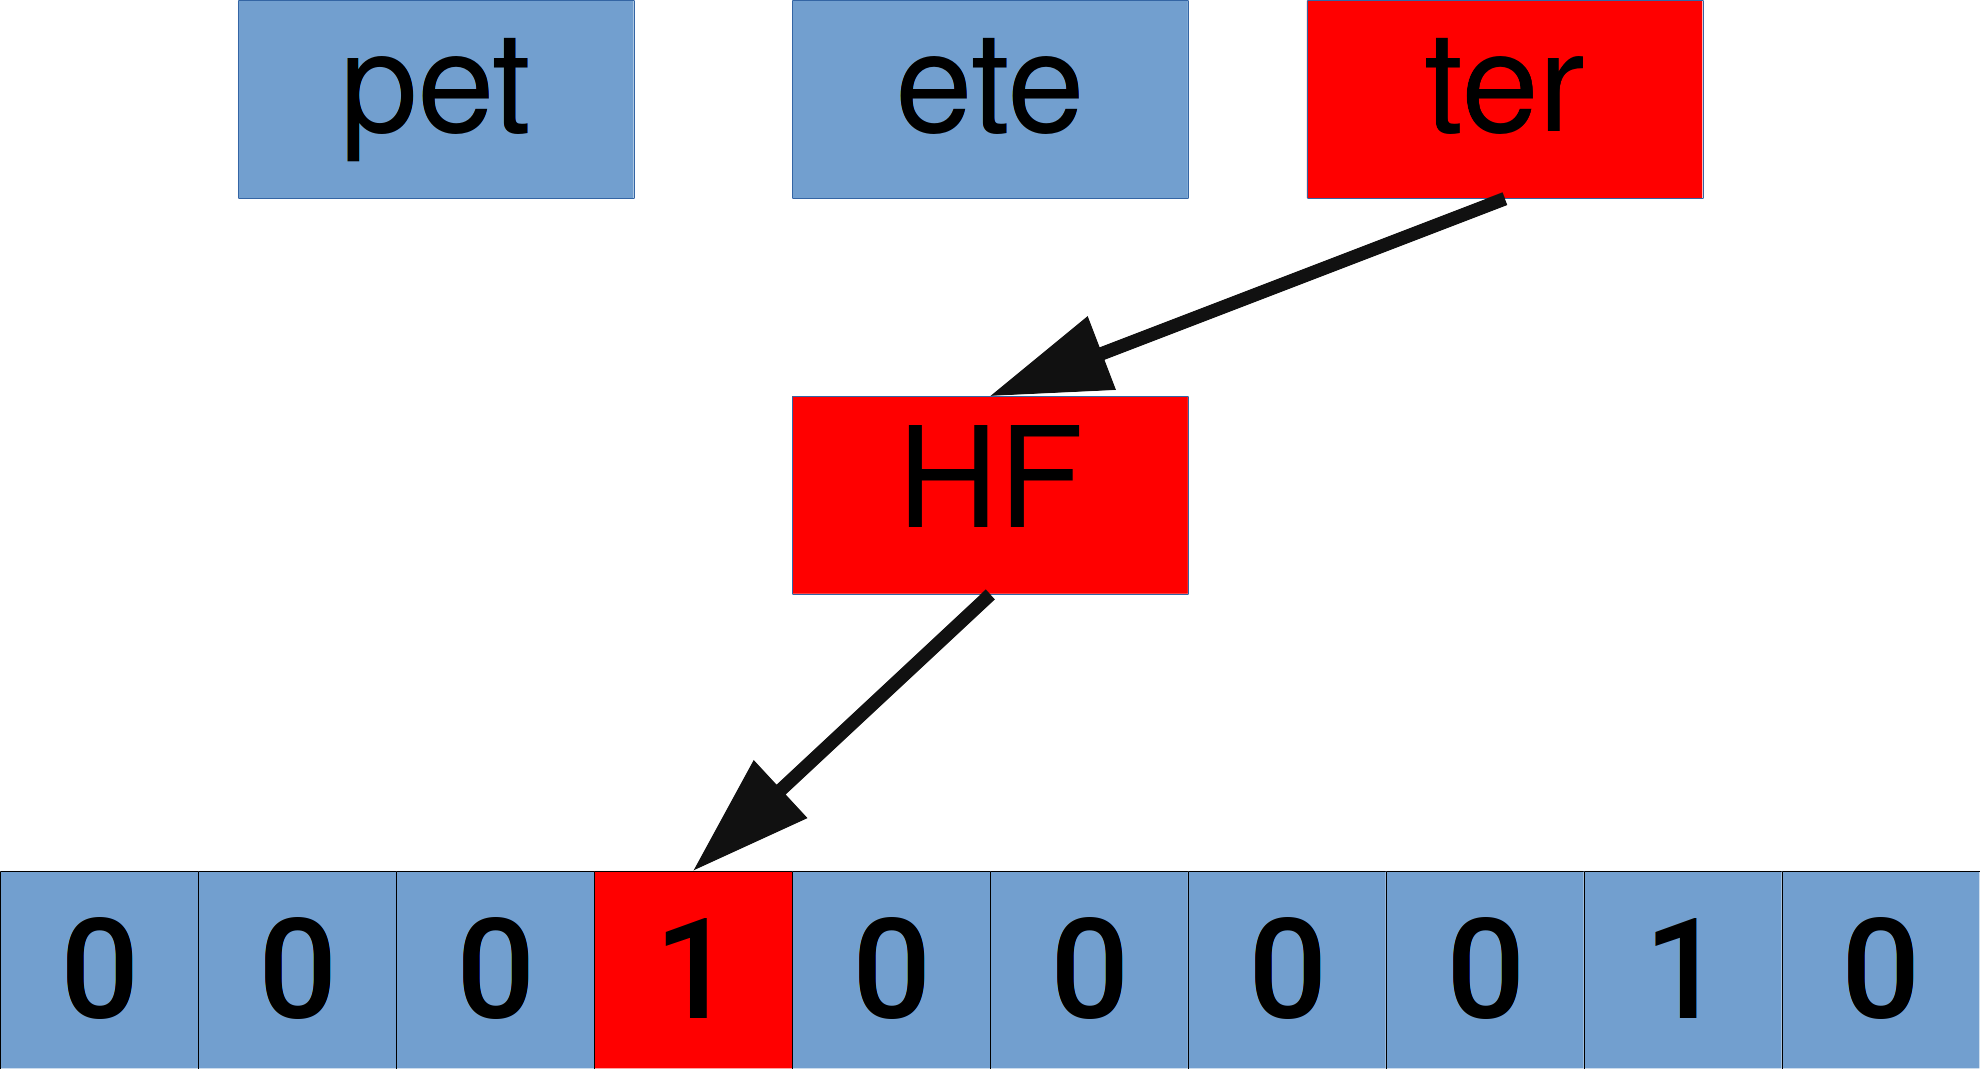
\includegraphics[width=0.9\textwidth]{Bilder/bloomfilter_example_insert_04.png}};
		\end{tikzpicture}
	}

	\begin{tikzpicture}[overlay]
		\node at (11.5, 1.5)
		{
			\begin{footnotesize}
			\begin{varwidth}{0.4\textwidth}
			\textbf{Hier:}
			\begin{itemize}
				\item Immer genau eine Hashfunktion!
			\end{itemize}
			\end{varwidth}
			\end{footnotesize}
		};
	\end{tikzpicture}
\end{frame}

\begin{frame}
	\vspace*{-0.1cm}
	\hspace*{-.35cm} \textbf{\underline{Transformation:}}
	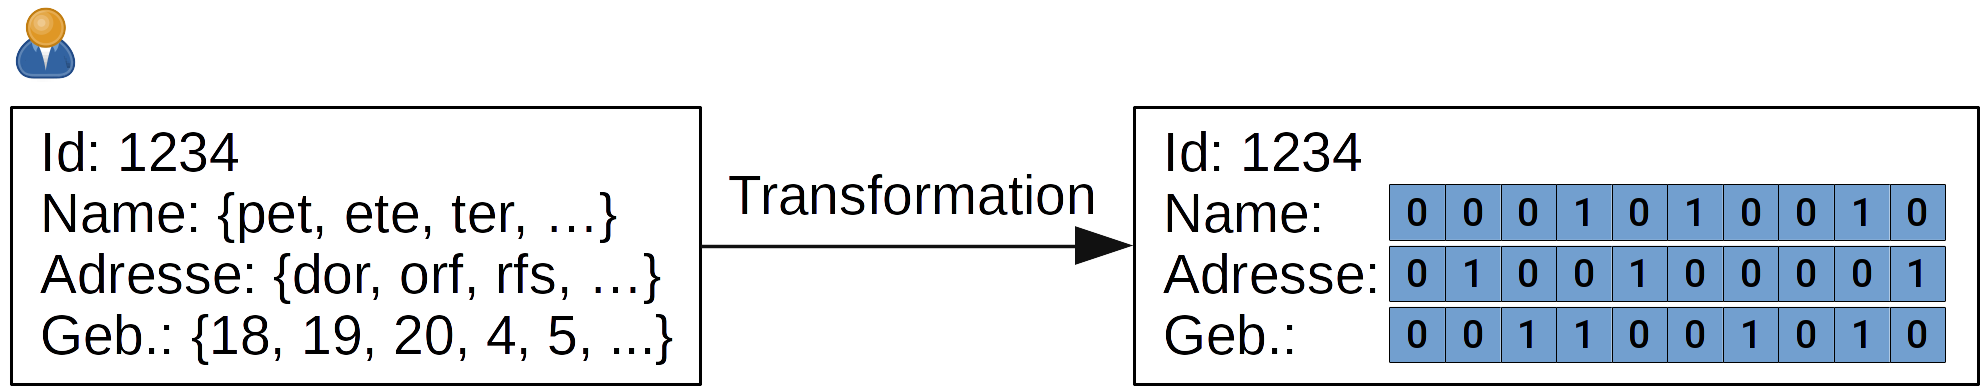
\includegraphics[width=1.01\textwidth]{Bilder/Transformation_Bitarray.png}
	\vspace*{0.5cm}

	\hspace*{-.35cm} \textbf{\underline{Ähnlichkeitsfunktion:}}
	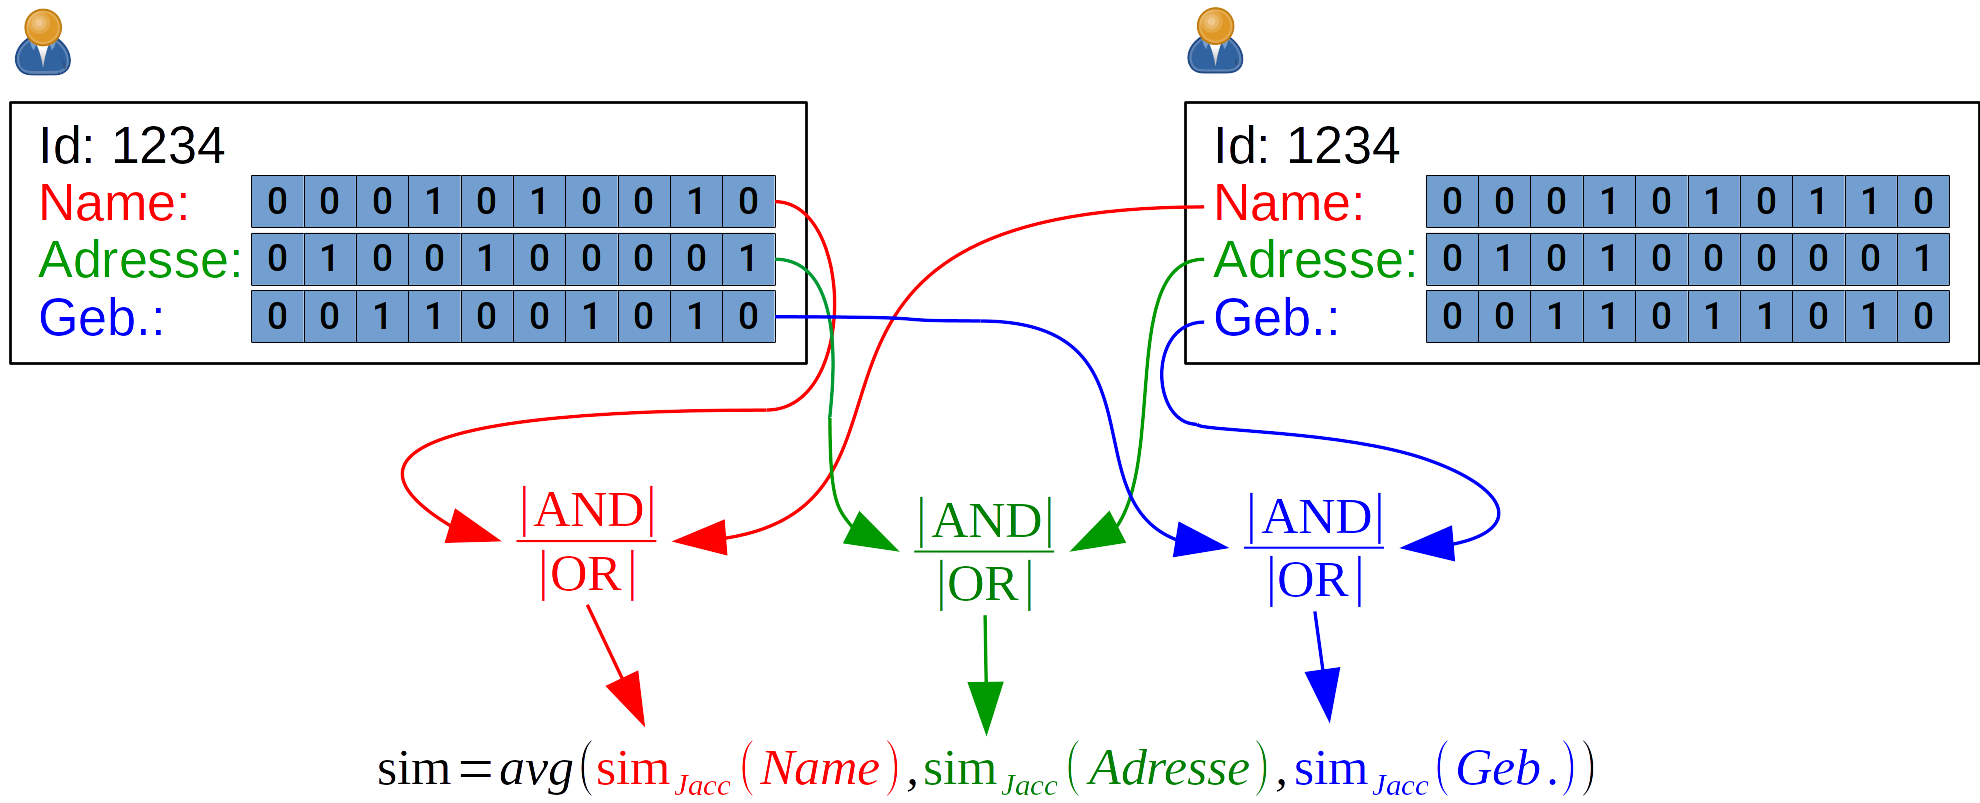
\includegraphics[width=1.01\textwidth]{Bilder/sim_bitarray.png}
\end{frame}

\subsection{Vergleich}
\begin{frame}
	\vspace*{-.025cm}
	\hspace*{-.5cm}
	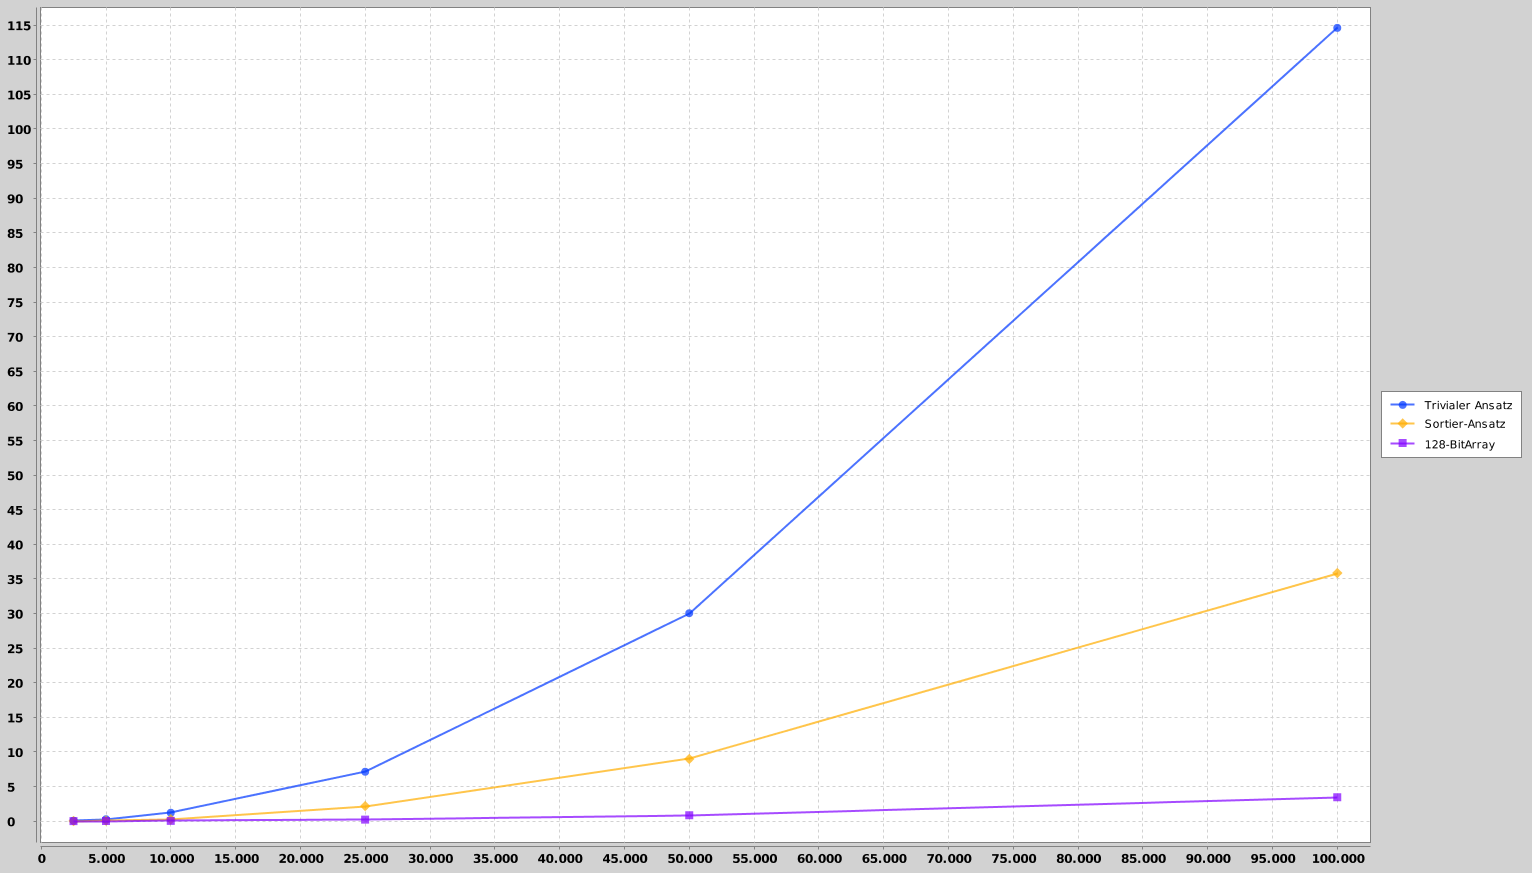
\includegraphics[width=1.07\textwidth, height=1.02\textheight]{Bilder/evaluation_runtime_for_threshold_0_7_trigram_one_fuzzy_date.png}

	\begin{tikzpicture}[overlay]
		\node at (4.7, 7)
		{
			\begin{footnotesize}
			\begin{varwidth}{0.75\textwidth}
			\textbf{Ausführungszeit in Minuten}
			\begin{itemize}
				\item für unterschiedlich große Datensätze
				\item Parameter
				\begin{itemize}
					\item Trigramme
					\item Threshold: $0.7$
					\item Datumsunschärfe: $1$
				\end{itemize}
				\item Testsystem
				\begin{itemize}
					\item CPU: 8 Kerne (HT) @ 3.4 GHz
					\item RAM: 16 GB
				\end{itemize}
			\end{itemize}
			\end{varwidth}
			\end{footnotesize}
		};
	\end{tikzpicture}

\end{frame}

\begin{frame}
	\vspace*{-.025cm}
	\hspace*{-.5cm}
	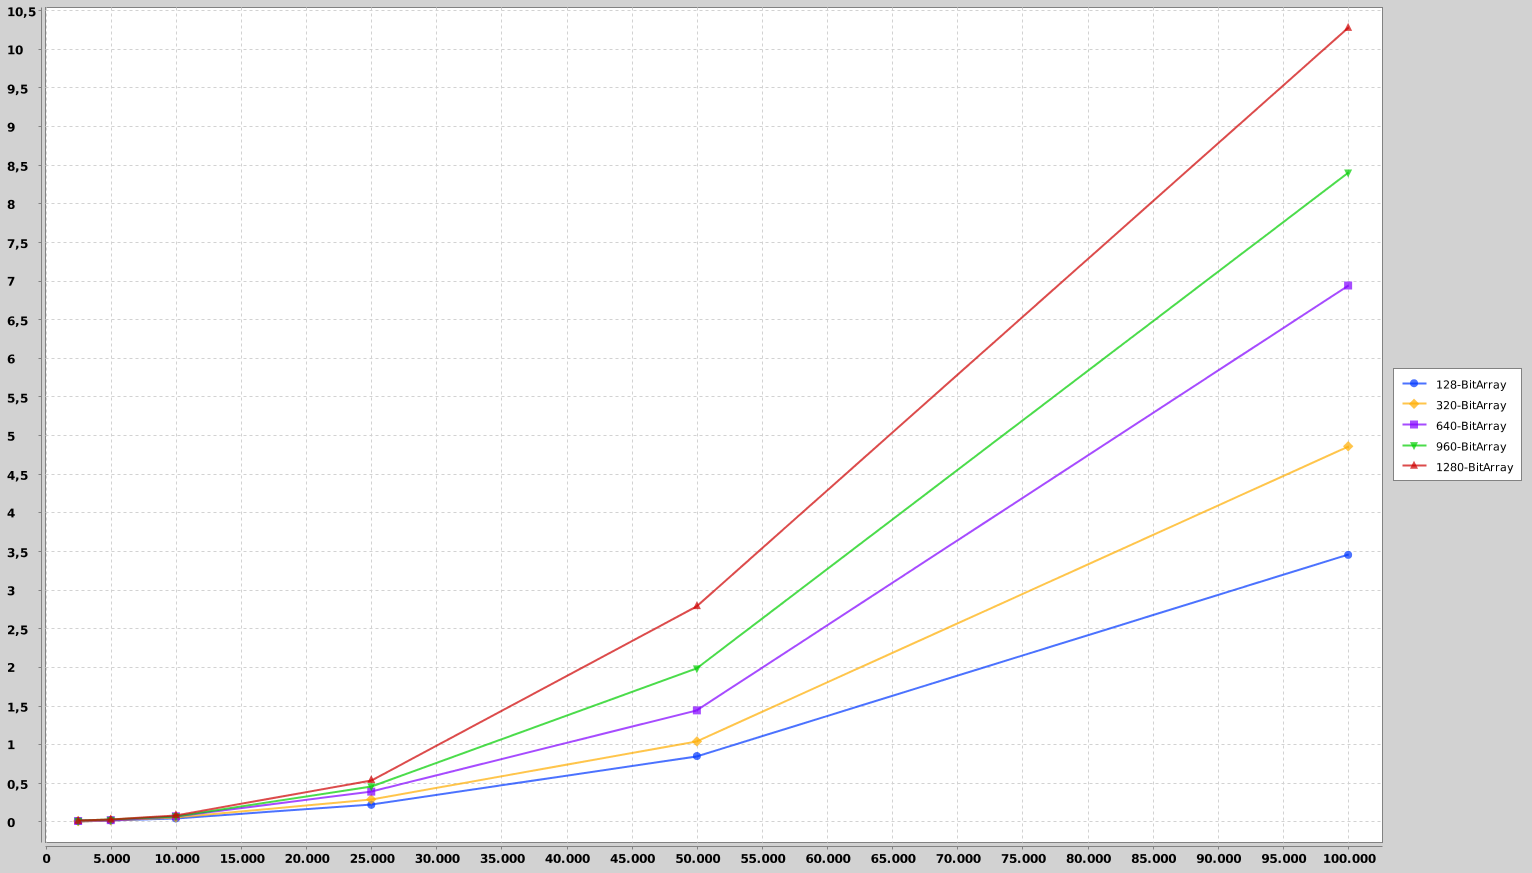
\includegraphics[width=1.07\textwidth, height=1.02\textheight]{Bilder/evaluation_runtime_bit_array_size_for_threshold_0_7_trigram_one_fuzzy_date.png}

	\begin{tikzpicture}[overlay]
		\node at (4.7, 7)
		{
			\begin{footnotesize}
			\begin{varwidth}{0.75\textwidth}
			\textbf{Ausführungszeit verschiedener Bit-Array-Größen in Minuten}
			\begin{itemize}
				\item für unterschiedlich große Datensätze
				\item Parameter
				\begin{itemize}
					\item Trigramme
					\item Threshold: $0.7$
					\item Datumsunschärfe: $1$
				\end{itemize}
				\item Testsystem
				\begin{itemize}
					\item CPU: 8 Kerne (HT) @ 3.4 GHz
					\item RAM: 16 GB
				\end{itemize}
			\end{itemize}
			\end{varwidth}
			\end{footnotesize}
		};
	\end{tikzpicture}

\end{frame}

\begin{frame}
	\hspace*{-.35cm} \textbf{\underline{Absolute Werte:}}
	\hspace*{-.5cm}
	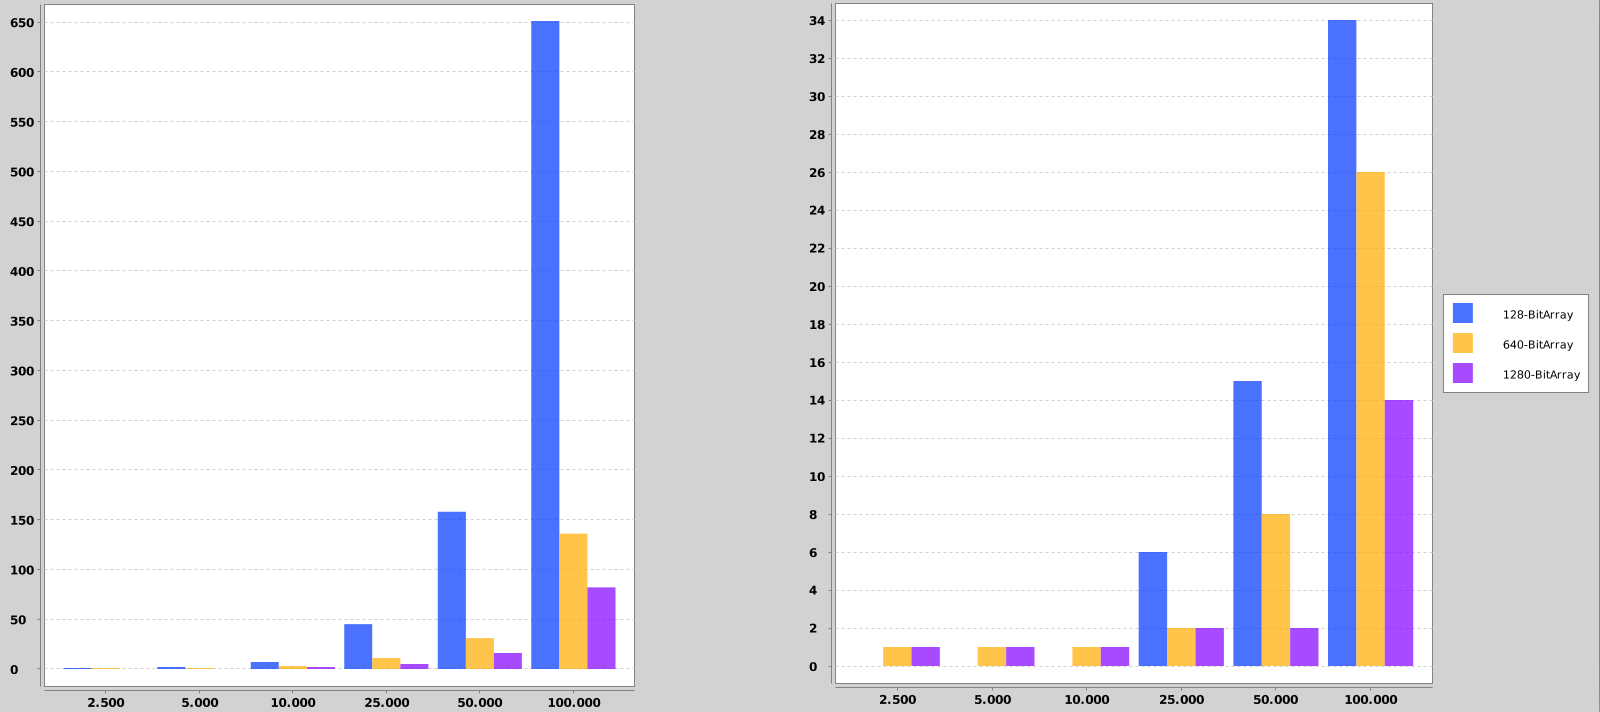
\includegraphics[width=1.07\textwidth, height=0.8\textheight]{Bilder/false_negative_false_positive_threshold_0_7_trigram_one_fuzzy_date.png}
	\begin{tikzpicture}[overlay]
		\node at (-10., 6)
		{
			\begin{footnotesize}
			\begin{varwidth}{0.4\textwidth}
			\textbf{False Positives}
			\begin{itemize}
				\item Trigramme
				\item Threshold: $0.7$
				\item Datumsunschärfe: $1$
			\end{itemize}
			\end{varwidth}
			\end{footnotesize}
		};

		\node at (-3.6, 6)
		{
			\begin{footnotesize}
			\begin{varwidth}{0.4\textwidth}
			\textbf{False Negatives}
			\begin{itemize}
				\item Trigramme
				\item Threshold: $0.7$
				\item Datumsunschärfe: $1$
			\end{itemize}
			\end{varwidth}
			\end{footnotesize}
		};

		\node (one) at (-12.2, 1) {\tiny $1$};
		\node (zero) at (-11.8, 1) {\tiny $0$};


		\node (a) at (-12.3, 0.32) {};
		\node (b) at (-12, 0.32) {};
		\node (c) at (-11.8, 0.32) {};

		\path [draw, ->] (one) -- (a);	
		\path [draw, ->] (one) -- (b);
		\path [draw, ->] (zero) -- (c);
	\end{tikzpicture}

	\uncover<2->
	{
		\begin{center}
		\begin{scriptsize}
		\begin{tabular}{l|c|c|c}
			& 128-Bit & 640-Bit & 1280-Bit\\
			\hline
			Precision & 0.955 & 0.990 & 0.994 \\
			\hline
			Recall & 0.998 & 0.998 & 0.999 \\
		\end{tabular}
		\end{scriptsize}
		\end{center}
		\begin{tikzpicture}[overlay]
			\node (a) at (10.7, 1.6) {};
			\node (b) at (9, 1) {};
			\node (c) at (4, 1.6) {};
			\node (d) at (4.7, 1) {};

			\path [draw, ->, green, very thick] (a) -- (b);	
			\path [draw, ->, green, very thick] (c) -- (d);	
		\end{tikzpicture}
	}
\end{frame}


\section{Optimierungen des Bit-Array-Ansatzes}

\subsection{Bit-Array als Filter}

\begin{frame}
	\setbeamercolor{normal text}{fg=gray,bg=}
	\setbeamercolor{alerted text}{fg=black,bg=}
	\usebeamercolor{normal text}

	\begin{itemize}
		\setlength\itemsep{\stdItemSep}
		\item \alert<1->{Zwischenschritt:}
		\begin{itemize}
			\setlength\itemsep{\stdItemSep}
			\vspace*{\stdItemSep}
			\item \alert<1->{Obere Schranke des Jaccard-Index mit Bit-Arrays effizient bestimmen}
		\end{itemize}
		\item \alert<2->{Idee:}
		\begin{itemize}
			\setlength\itemsep{\stdItemSep}
			\vspace*{\stdItemSep}
			\item \alert<2->{$A$, $B$ - Mengen}
			\item \alert<3->{$A_{F}$ $=$ $bloom(A)$, $B_{F}$ $=$ $bloom(B)$ - Bit-Arrays der Mengen}
			\item \alert<4->{Es gilt:}
			\begin{itemize}
				\setlength\itemsep{\stdItemSep}
				\vspace*{\stdItemSep}
				\item \alert<4->{$|A_{F}|$ $\leq$ $|A|$}
				\item \alert<5->{$|A_{F} \vee B_{F}|$ $\leq$ $|A \cup B|$}
				\item \alert<6->{$jaccard(A, B)$ $=$ $\frac{|A \cap B|}{|A \cup B|}$} \alert<7->{$=$ $\frac{|A| + |B| - |A \cup B|}{|A \cup B|}$}
					\alert<8->{$\leq$ $\frac{|A| + |B| - |A_{F} \vee B_{F}|}{|A_{F} \vee B_{F}|}$}
			\end{itemize}
		\end{itemize}
		\item \alert<9->{Vorgehen:}
		\begin{itemize}
			\setlength\itemsep{\stdItemSep}
			\vspace*{\stdItemSep}
			\item \alert<9->{Schätze Jaccard-Index}
			\item \alert<10->{Größer Threshold? $\Rightarrow$ berechne Jaccard-Index}
		\end{itemize}
	\end{itemize}

	\uncover<9->
	{
		\begin{tikzpicture}[overlay]
			\node (start) at (2.5, 1.5) {};
			\node (end) at (8.7, 2.5) {};
			\path [draw, ->, green, very thick] (start) -- (end);
		\end{tikzpicture}
	}
	\uncover<10->
	{
		\begin{tikzpicture}[overlay]
			\node (start) at (5.5, 0.8) {};
			\node (end) at (6, 2.5) {};
			\path [draw, ->, blue, very thick] (start) -- (end);
		\end{tikzpicture}
	}
\end{frame}

\begin{frame}
	\vspace*{-.025cm}
	\hspace*{-.5cm}
	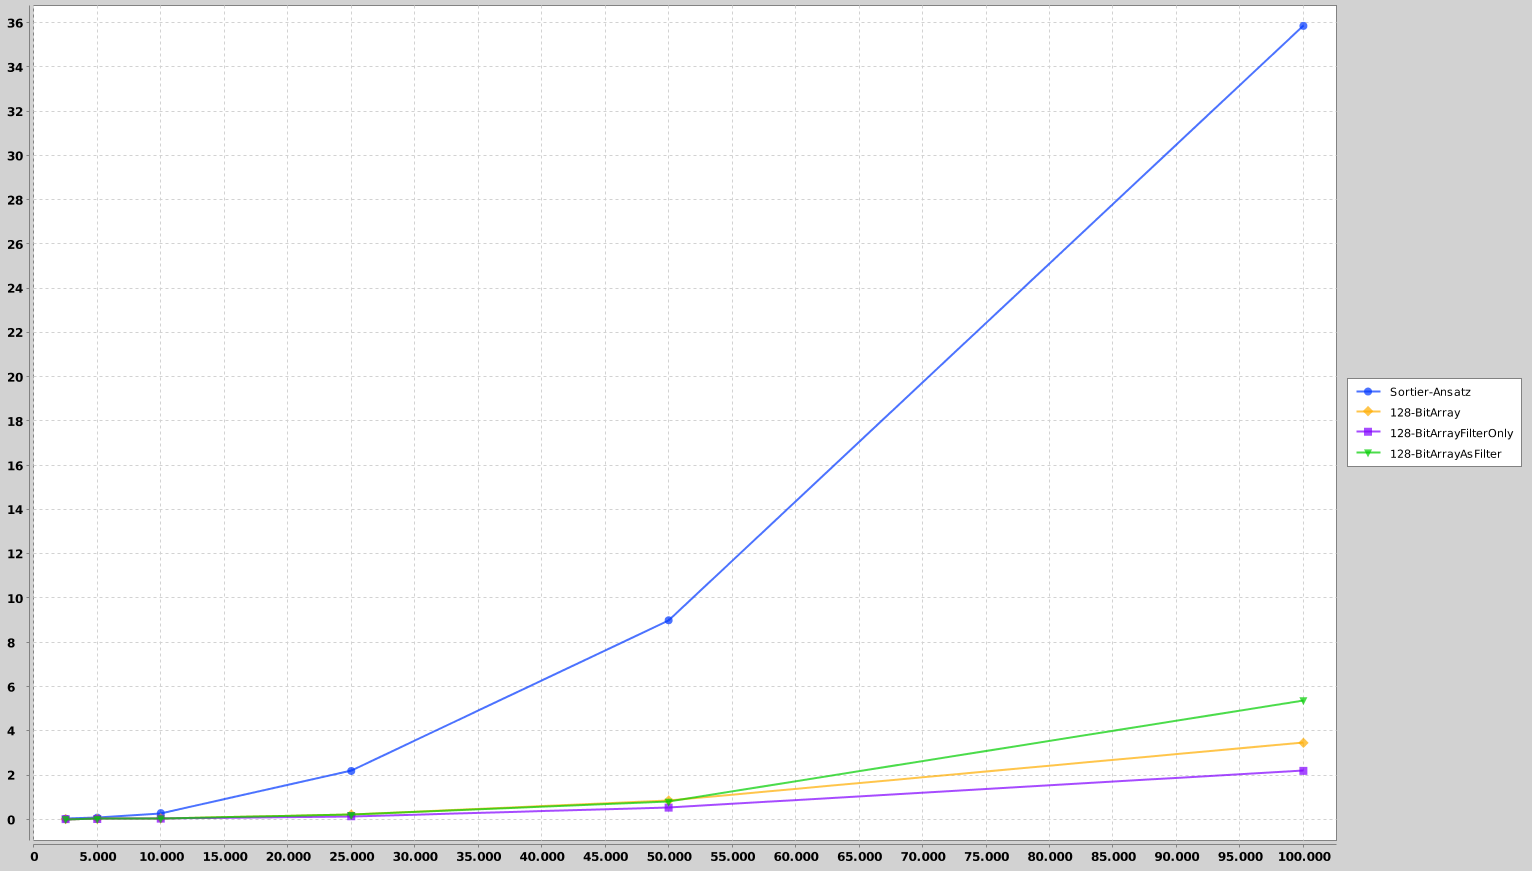
\includegraphics[width=1.07\textwidth, height=1.02\textheight]{Bilder/second_runtime_evaluation_for_threshold_0_7_trigram_one_fuzzy_date.png}

	\begin{tikzpicture}[overlay]
		\node at (3.6, 7)
		{
			\begin{footnotesize}
			\begin{varwidth}{0.6\textwidth}
			\textbf{Ausführungszeit in Minuten}
			\begin{itemize}
				\item für unterschiedlich große Datensätze
				\item Parameter
				\begin{itemize}
					\item Trigramme
					\item Threshold: $0.7$
					\item Datumsunschärfe: $1$
				\end{itemize}
				\item Testsystem
				\begin{itemize}
					\item CPU: 8 Kerne (HT) @ 3.4 GHz
					\item RAM: 16 GB
				\end{itemize}
			\end{itemize}
			\end{varwidth}
			\end{footnotesize}
		};
	\end{tikzpicture}

\end{frame}

\subsection{Filtern in 2 Phasen}

\begin{frame}
	\frametitle{Filtern in 2 Phasen}
	\begin{itemize}
		\setlength\itemsep{\stdItemSep}
		\item Phase 1
		\begin{itemize}
			\setlength\itemsep{\stdItemSep}
			\vspace*{\stdItemSep}
			\item ER mit Bit-Array-Filter-Only
		\end{itemize}
		\item Phase 2
		\begin{itemize}
			\setlength\itemsep{\stdItemSep}
			\vspace*{\stdItemSep}
			\item Eingabe: Id-Paare der Kandidaten aus Phase 1
			\item Import (Normalisierung + Transformation) für Sortier-Ansatz aus
			\item ER nur für Kandidaten-Paare
		\end{itemize}
	\end{itemize}
\end{frame}

\begin{frame}
	\vspace*{-.025cm}
	\hspace*{-.5cm}
	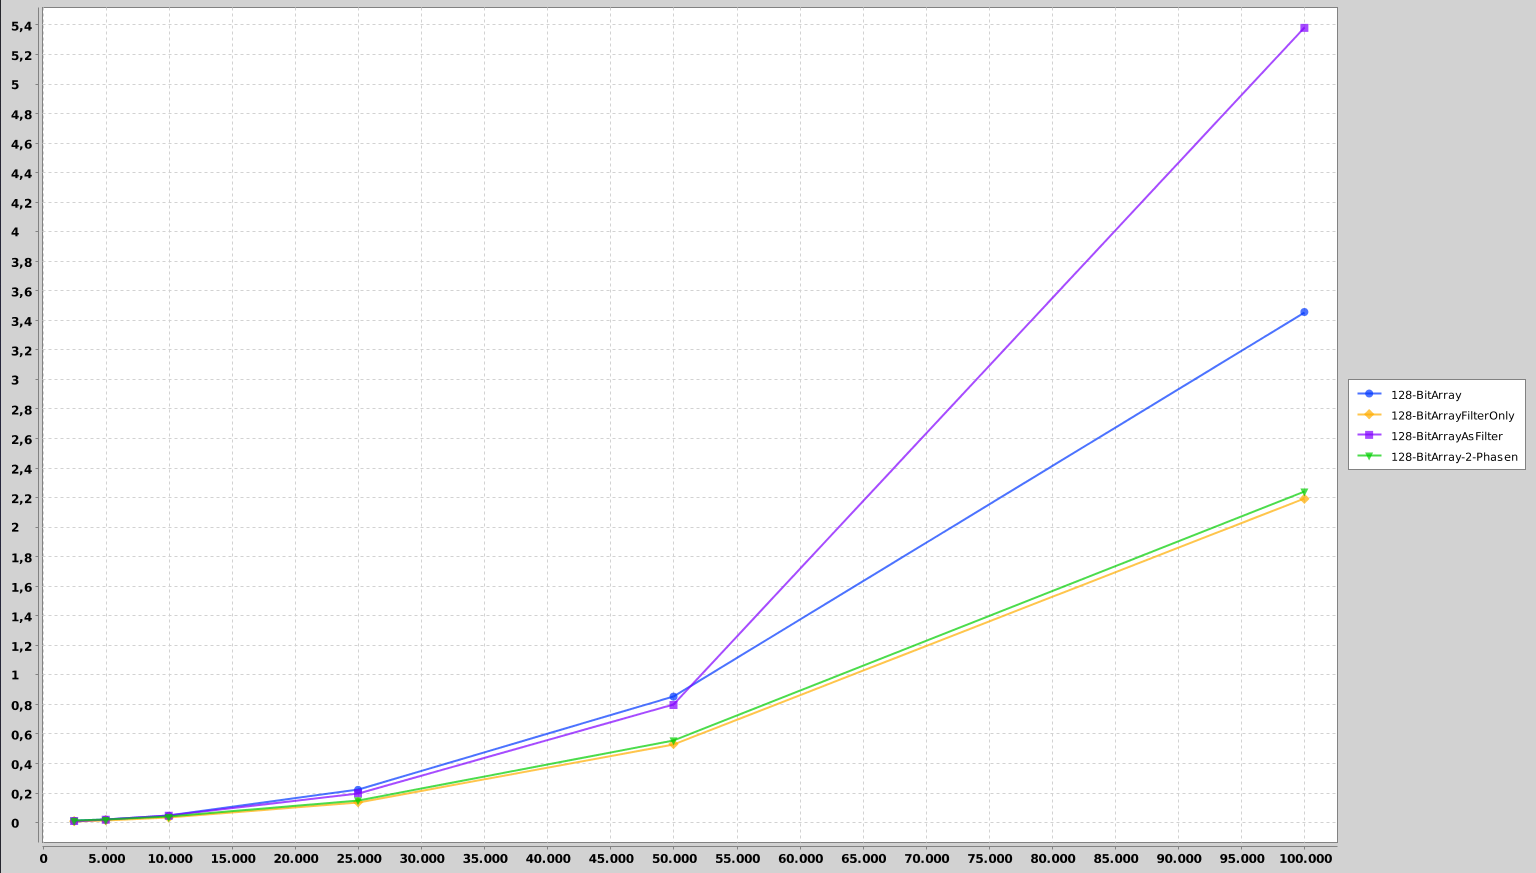
\includegraphics[width=1.07\textwidth, height=1.02\textheight]{Bilder/final_comparison_bit_array_approaches__threshold_0_7_trigram_one_fuzzy_date.png}

	\begin{tikzpicture}[overlay]
		\node at (3.65, 7)
		{
			\begin{footnotesize}
			\begin{varwidth}{0.6\textwidth}
			\textbf{Ausführungszeit in Minuten}
			\begin{itemize}
				\item für unterschiedlich große Datensätze
				\item Parameter
				\begin{itemize}
					\item Trigramme
					\item Threshold: $0.7$
					\item Datumsunschärfe: $1$
				\end{itemize}
				\item Testsystem
				\begin{itemize}
					\item CPU: 8 Kerne (HT) @ 3.4 GHz
					\item RAM: 16 GB
				\end{itemize}
			\end{itemize}
			\end{varwidth}
			\end{footnotesize}
		};
	\end{tikzpicture}
\end{frame}


\section{Rückblick + Ausblick}

\begin{frame}
	\begin{itemize}
		\setlength\itemsep{\stdItemSep}
		\item Erfahrungen:
		\begin{itemize}
			\setlength\itemsep{\stdItemSep}
			\vspace*{\stdItemSep}
			\item Abstraktion + große Datenstrukturen sind teuer
		\end{itemize}
		\item Tipps für unbekannte Datensätze:
		\begin{itemize}
			\setlength\itemsep{\stdItemSep}
			\vspace*{\stdItemSep}
			\item Untersuche Datensatz mit \glqq Phase 1\grqq
			\item Schrittweise Anpassung der Parameter
			\begin{itemize}
				\setlength\itemsep{\stdItemSep}
				\vspace*{\stdItemSep}
				\item Ziel: sehr hohe Selektivität trotz kleinem Bit-Array
			\end{itemize}
			\item Abschließend: ER mit \glqq Phase 1 + 2\grqq
		\end{itemize}
		\item mögliche Nächste Schritte:
		\begin{itemize}
			\setlength\itemsep{\stdItemSep}
			\vspace*{\stdItemSep}
			\item Parallelisierung
			\item Ein Partitionierter Bit-Array
			\item Vergleich mit weiteren ER-Ansätzen
			\item Integration unterschiedlicher ER-Ansätze als \glqq Phase 2\grqq
		\end{itemize}
	\end{itemize}
\end{frame}


\end{document}
